% PDF p. 63
\section{黎曼度量的张量记法}
\subsection{张量积}
第~\ref{ch:03}~章将讨论张量积（tensor product）。这里先作简要说明。

\subsubsection{张量积的定义}
设 $M$ 为光滑流形，局部坐标为 $(x^1,\ldots,x^n)$。对每一坐标 $x^i$，其微分
\[
  dx^i\colon T_pM\longrightarrow\R,\qquad dx^i(v)=v[x^i],
\]
% PDF p. 64
是一个\textbf{1-形式}（one-form），即 $(0,1)$ 型协变张量。它与另一个 1-形式 $dx^j$ 的张量积是 $(0,2)$ 型张量
\[
  (dx^i\otimes dx^j)(u,v)=dx^i(u)\,dx^j(v),\qquad u,v\in T_pM.
\]
也就是说，将第一自变量 $u$ 代入第一因子，将第二自变量 $v$ 代入第二因子，再将所得的两个数相乘。

\subsubsection{坐标表示}
用坐标基表示切向量
\[
  u=u^k\partial_{x^k},\qquad v=v^l\partial_{x^l}.
\]
因为 $dx^i(\partial_{x^k})=\delta^i_k$，所以
\[
  (dx^i\otimes dx^j)(u,v)=u^i v^j.
\]
于是，$dx^i\otimes dx^j$ 就是一个基本矩阵，从 $u$ 中选出第 $i$ 个分量，从 $v$ 中选出第 $j$ 个分量。

\subsubsection{黎曼度量}
回顾式~\eqref{eq:2.4}，黎曼度量满足
\begin{equation*}
  g_p(u,v)=\sum_i\sum_j g_{ij}(p)u^iv^j.
  \tag{2.15}\label{eq:2.15}
\end{equation*}
利用式（6）\translatornote{原书在此将式~\eqref{eq:2.6} 简称为“(6)”。下式求和项中的两处上标 $i$ 依原书保留。按求和指标应改为 $j$。} 得
\begin{equation*}
  dx^i(u)=dx^i\!\left(\sum_j u^i\frac{\partial}{\partial x^i}\right)=u^i.
  \tag{2.16}\label{eq:2.16}
\end{equation*}
类似地，
\begin{equation*}
  dx^j(v)=v^j.
  \tag{2.17}\label{eq:2.17}
\end{equation*}
将式~\eqref{eq:2.16}、\eqref{eq:2.17} 与张量积的定义结合起来，得到
\begin{equation*}
  (dx^i\otimes dx^j)(u,v)=dx^i(u)\,dx^j(v)=u^iv^j.
  \tag{2.18}\label{eq:2.18}
\end{equation*}
把式~\eqref{eq:2.18} 代入式~\eqref{eq:2.15}，得到
\begin{equation*}
  g_p(u,v)=\sum_i\sum_j g_{ij}(p)(dx^i\otimes dx^j)(u,v).
  \tag{2.19}\label{eq:2.19}
\end{equation*}
用对偶基 1-形式 $dx^i$ 表示，度量张量（metric tensor）$g$ 可写为
\begin{equation*}
  g=g_{ij}\,dx^i\otimes dx^j.
  \tag{2.20}\label{eq:2.20}
\end{equation*}

% PDF p. 65
这个表达式将度量表示为二阶张量，即二阶协变张量。若 $dx^i\,dx^j$ 表示只使用 $x^1$ 和 $x^2$ 两个坐标的\textbf{局部坐标基}，则度量在局部二维坐标系中化为
\begin{equation*}
  g=g_{ij}\,dx^i\,dx^j.
  \tag{2.21}\label{eq:2.21}
\end{equation*}

\section{换标架时的黎曼度量}
现在研究改变局部坐标时，黎曼度量的计算公式如何变化。设 $(U',\varphi'=(x^{1'},\ldots,x^{n'}))$ 是 $M$ 的另一张坐标卡，且 $U\cap U'\neq\varnothing$。由链式法则得到
\begin{equation*}
  \frac{\partial}{\partial x^{i'}}
  =\sum_k \frac{\partial x^k}{\partial x^{i'}}\frac{\partial}{\partial x^k}.
  \tag{2.22}\label{eq:2.22}
\end{equation*}
于是，根据黎曼度量的定义及式~\eqref{eq:2.22}，得到 $g$ 关于 $(U,\varphi)$ 与 $(U',\varphi')$ 的局部表示之间的关系
\begin{equation*}
  \begin{aligned}
    g_{i'j'}&=g\!\left(\frac{\partial}{\partial x^{i'}},\frac{\partial}{\partial x^{j'}}\right)\\
    &=g\!\left(\sum_k\frac{\partial x^k}{\partial x^{i'}}\frac{\partial}{\partial x^k},
         \sum_l\frac{\partial x^l}{\partial x^{j'}}\frac{\partial}{\partial x^l}\right)\\
    &=\sum_k\sum_l\frac{\partial x^k}{\partial x^{i'}}\frac{\partial x^l}{\partial x^{j'}}\,g_{kl}.
  \end{aligned}
  \tag{2.23}\label{eq:2.23}
\end{equation*}

\begin{statement}{例 2.3}{欧氏度量与极坐标}
标准欧氏度量用笛卡儿坐标表示。利用式~\eqref{eq:2.4}，得到
\begin{equation*}
  \begin{aligned}
    g_{11}&=g_p\!\left(\frac{\partial}{\partial x},\frac{\partial}{\partial x}\right)=1,\\
    g_{12}&=g_{21}=g_p\!\left(\frac{\partial}{\partial x},\frac{\partial}{\partial y}\right)=0,\\
    g_{22}&=g_p\!\left(\frac{\partial}{\partial y},\frac{\partial}{\partial y}\right)=1.
  \end{aligned}
  \tag{2.24}\label{eq:2.24}
\end{equation*}
利用式~\eqref{eq:2.21} 与式~\eqref{eq:2.24}，得到 $g=(dx)^2+(dy)^2=dx^2+dy^2$。一般地，欧氏空间为 $\R^n$。在自然等同 $T_x\R^n=\R^n$ 下，欧氏度量 $\bar g$ 就是各切空间上的通常内积。在标准坐标下，$\bar g$ 可写成
\begin{equation*}
  \bar g=\bar g_{ij}\,dx^i\,dx^j,
  \tag{2.25}\label{eq:2.25}
\end{equation*}
其中 $\bar g_{ij}=\delta_{ij}$。

\textbf{考虑极坐标。}令 $x=r\cos\theta$，$y=r\sin\theta$，则
\begin{equation*}
  \begin{aligned}
    \frac{\partial x}{\partial r}&=\cos\theta,&
    \frac{\partial x}{\partial\theta}&=-r\sin\theta,\\
    \frac{\partial y}{\partial r}&=\sin\theta,&
    \frac{\partial y}{\partial\theta}&=r\cos\theta.
  \end{aligned}
  \tag{2.26}\label{eq:2.26}
\end{equation*}
% PDF p. 66
利用式~\eqref{eq:2.23} 与式~\eqref{eq:2.26}，得到
\begin{equation*}
  \begin{aligned}
    g_{r,r}
      &=\left(\frac{\partial x}{\partial r}\right)^2
        +\left(\frac{\partial y}{\partial r}\right)^2
        =\cos^2\theta+\sin^2\theta=1,\\
    g_{r,\theta}=g_{\theta,r}
      &=\frac{\partial x}{\partial r}\frac{\partial x}{\partial\theta}
        +\frac{\partial y}{\partial r}\frac{\partial y}{\partial\theta}\\
      &=\cos\theta(-r\sin\theta)+\sin\theta(r\cos\theta)=0,\\
    g_{\theta,\theta}
      &=\left(\frac{\partial x}{\partial\theta}\right)^2
        +\left(\frac{\partial y}{\partial\theta}\right)^2\\
      &=(-r\sin\theta)^2+(r\cos\theta)^2=r^2.
  \end{aligned}
  \tag{2.27}\label{eq:2.27}
\end{equation*}
由式~\eqref{eq:2.21} 与式~\eqref{eq:2.27} 得
\begin{equation*}
  g=(dr)^2+r^2(d\theta)^2=dr^2+r^2d\theta^2.
  \tag{2.28}\label{eq:2.28}
\end{equation*}
\end{statement}

\section{黎曼子流形与等距浸入}
下面介绍黎曼度量的其他例子，包括子流形及乘积流形。先考虑浸入子流形。

\begin{statement}{定义 2.6}{黎曼子流形}
设 $(M,g)$ 是黎曼流形，$\iota\colon N\to M$ 给出浸入子流形（immersed submanifold）。换言之，$N$ 是光滑流形，$\iota$ 是单射浸入。$g$ 在 $N$ 上诱导的黎曼度量 $g_N$ 定义如下。设 $p\in M$。\translatornote{原书此处写作 $p\in M$，以下 $d\iota_p$ 以 $p\in N$ 为定义域中的基点。} 通过单射 $d\iota_p\colon T_pN\to T_{\iota(p)}M$，可将切空间 $T_pN$ 视为 $M$ 中相应切空间的子空间。$N$ 上的黎曼度量 $g_N$ 是 $g$ 在 $N$ 上的限制，定义为
\begin{equation*}
  g_N(u,v)=g(u,v),\qquad \forall u,v\in T_pN,
  \tag{2.29}\label{eq:2.29}
\end{equation*}
也可把 $(g_N)_p$ 定义为
\begin{equation*}
  (g_N)_p(u,v)=g_{\iota(p)}\bigl(d\iota_p(u),d\iota_p(v)\bigr),
  \tag{2.30}\label{eq:2.30}
\end{equation*}
其中 $u,v\in T_pN$。

若 $\iota$ 是浸入，但不一定是单射，仍称 $g_N$ 为拉回度量，写作 $g_N=\iota^*g$，并称 $\iota\colon(N,g_N)\to(M,g)$ 为\textbf{等距浸入}（isometric immersion）。当然，任一浸入都必定局部单射。
\end{statement}

% PDF p. 67
\section{乘积黎曼流形}
设 $(M_1,g_1)$ 和 $(M_2,g_2)$ 是两个黎曼流形，$M_1\times M_2$ 是光滑乘积流形（图~\ref{fig:2.2}）。在它上面有一个典范的黎曼度量 $g$，称为乘积黎曼度量（product Riemannian metric），其定义如下。设 $p=(p_1,p_2)\in M_1\times M_2$，其中 $p_1\in M_1$、$p_2\in M_2$。那么 $M$ 在 $p$ 处的切空间可写成\textbf{直和}
$T_pM=T_{p_1}M_1\oplus T_{p_2}M_2$（图~\ref{fig:2.3}）。

设 $u_1,v_1\in T_{p_1}M_1$、$u_2,v_2\in T_{p_2}M_2$，且 $u=u_1+u_2$、$v=v_1+v_2$。给定 $u,v\in T_pM$，定义
\begin{equation*}
  g_p(u,v)=g_{p_1}(u_1,v_1)+g_{p_2}(u_2,v_2).
  \tag{2.31}\label{eq:2.31}
\end{equation*}

\begin{figure}[htbp]
  \centering
  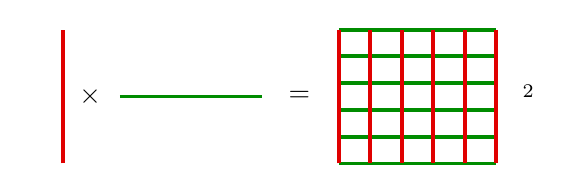
\begin{tikzpicture}[x=1cm,y=1cm]
  \draw[red!88!black,line width=1.4pt] (0,-.85)--(0,.85);
  \node[left=6pt] at (0,0) {$\R$};
  \node at (.34,0) {$\times$};
  \draw[green!55!black,line width=1.4pt] (.72,0)--(2.52,0)
       node[midway,below=2pt] {$\R$};
  \node at (3,0) {$=$};
  \foreach \y in {-.85,-.51,-.17,.17,.51,.85}
     \draw[green!55!black,line width=1.4pt] (3.5,\y)--(5.5,\y);
  \foreach \x in {3.5,3.9,4.3,4.7,5.1,5.5}
     \draw[red!88!black,line width=1.4pt] (\x,-.85)--(\x,.85);
  \node[right=6pt] at (5.5,0) {$\R^2$};
\end{tikzpicture}

  \FigureCaption{2.2}{流形的笛卡儿积示意图。}
\end{figure}

\begin{figure}[htbp]
  \centering
  \begin{tikzpicture}[x=.94cm,y=.94cm,>=Stealth]
  \foreach \i in {1,...,11}
    \foreach \j in {1,...,11}
      \fill[black!9] (.59*\i,.59*\j) circle (1pt);
  \draw[->,thick] (-.3,0)--(7.1,0) node[below right] {$M_1$};
  \draw[->,thick] (0,-.3)--(0,7.0) node[above left] {$M_2$};
  \coordinate (p) at (3.8,3.28);
  \draw[->,line width=1.5pt,blue!70!black] (p)--++(1.95,0)
       node[above right] {$v_1\in T_{p_1}M_1$};
  \draw[->,line width=1.5pt,green!50!black] (p)--++(0,1.95)
       node[above right] {$v_2\in T_{p_2}M_2$};
  \draw[->,line width=1.5pt,red!87!black] (p)--++(1.95,1.95)
       node[below right] {$v_1\oplus v_2$};
  \draw[thick] ([shift={(-3pt,-3pt)}]p)--([shift={(3pt,3pt)}]p)
       ([shift={(-3pt,3pt)}]p)--([shift={(3pt,-3pt)}]p);
  \node[above right,inner sep=2pt] at (p) {$p=(p_1,p_2)$};
\end{tikzpicture}

  \FigureCaption{2.3}{乘积流形 $M=M_1\times M_2$ 的切空间 $T_pM=T_{p_1}M_1\oplus T_{p_2}M_2$。}
\end{figure}

% PDF p. 68
设 $(x^1,\ldots,x^n)$ 是 $M_1$ 的局部坐标，$(x^{n+1},\ldots,x^{n+m})$ 是 $M_2$ 的局部坐标。那么 $(x^1,\ldots,x^{n+m})$ 是乘积流形 $M_1\times M_2$ 的坐标。$M_1\times M_2$ 上的黎曼度量为 $g=g_{ij}\,dx^i\,dx^j$，其中 $(g_{ij})$ 是分块对角矩阵
\begin{equation*}
  (g_{ij})=\begin{pmatrix}(g_1)_{ij}&0\\0&(g_2)_{ij}\end{pmatrix}.
  \tag{2.32}\label{eq:2.32}
\end{equation*}
显然，$g$ 是黎曼度量。由定义可知，$T_{p_1}M_1\oplus\{0\}$ 与 $\{0\}\oplus T_{p_2}M_2$ 正交。有时可记作 $(M,g)=(M_1,g_1)\times(M_2,g_2)$ 或 $g=g_1+g_2$。显然，欧氏空间 $\R^n$ 可视为 $n$ 个 $\R$ 的黎曼乘积。
